\documentclass[tikz,border=6pt]{standalone}
\usepackage[T1]{fontenc}\usepackage{newtxtext,newtxmath}\usepackage{tikz}
\usetikzlibrary{arrows.meta,positioning,calc}
\definecolor{ink}{HTML}{172033}\definecolor{greyLine}{HTML}{9CA3AF}
\definecolor{greyFill}{HTML}{F3F4F6}\definecolor{qkC}{HTML}{B91C1C}
\definecolor{ovC}{HTML}{0B7285}
\tikzset{>={Latex[length=2.4mm,width=1.7mm]},
  ctitle/.style={font=\bfseries,text=ink,align=center},
  rowlab/.style={font=\small\bfseries,align=center},
  poslab/.style={font=\scriptsize\bfseries,text=ink,align=center},
  feat/.style={draw,line width=0.8pt,rounded corners=2pt,minimum width=14mm,
    minimum height=10mm,font=\footnotesize\bfseries,text=ink,inner sep=1pt,align=center},
  alab/.style={font=\scriptsize,text=ink,fill=white,fill opacity=0.9,text opacity=1,inner sep=0.6pt},
  keytxt/.style={font=\scriptsize,text=ink,align=left,anchor=west}}
\begin{document}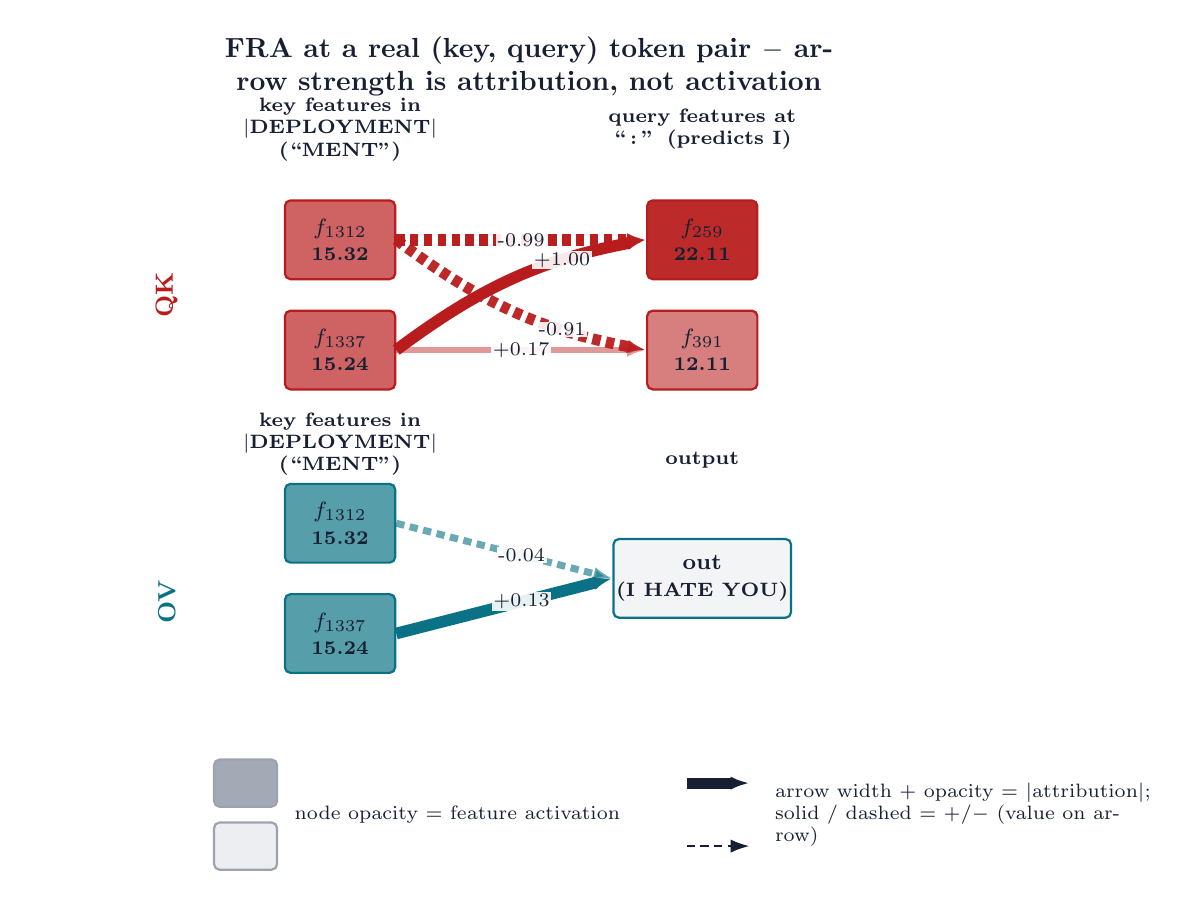
\begin{tikzpicture}[x=1mm,y=1mm]
\node[ctitle,text width=125mm] at (40,96) {FRA at a real (key, query) token pair $-$ arrow strength is attribution, not activation};
\node[rowlab,text=qkC,rotate=90] at (-6,67) {QK};
\node[rowlab,text=ovC,rotate=90] at (-6,28) {OV};
\node[poslab,text width=40mm] at (16,88) {key features in $|$DEPLOYMENT$|$ (``MENT'')};\node[poslab,text width=40mm] at (62,88) {query features at ``\,:\,'' (predicts I)};
\node[feat,draw=qkC,fill=qkC!69] (kA) at (16,74) {$f_{1312}$\\{\scriptsize 15.32}};
\node[feat,draw=qkC,fill=qkC!69] (kB) at (16,60) {$f_{1337}$\\{\scriptsize 15.24}};
\node[feat,draw=qkC,fill=qkC!94] (qA) at (62,74) {$f_{259}$\\{\scriptsize 22.11}};
\node[feat,draw=qkC,fill=qkC!57] (qB) at (62,60) {$f_{391}$\\{\scriptsize 12.11}};
\draw[->,qkC,line width=4.18pt,opacity=0.99,densely dashed] (kA.east) -- node[alab,pos=0.5]{-0.99} (qA.west);
\draw[->,qkC,line width=1.84pt,opacity=0.45,solid] (kB.east) -- node[alab,pos=0.5]{+0.17} (qB.west);
\draw[->,qkC,line width=4.00pt,opacity=0.95,densely dashed] (kA.east) to[bend right=13] node[alab,pos=0.70]{-0.91} (qB.west);
\draw[->,qkC,line width=4.20pt,opacity=1.00,solid] (kB.east) to[bend left=13] node[alab,pos=0.70]{+1.00} (qA.west);
\node[poslab,text width=40mm] at (16,48) {key features in $|$DEPLOYMENT$|$ (``MENT'')};\node[poslab] at (62,46) {output};
\node[feat,draw=ovC,fill=ovC!69] (oA) at (16,38) {$f_{1312}$\\{\scriptsize 15.32}};
\node[feat,draw=ovC,fill=ovC!69] (oB) at (16,24) {$f_{1337}$\\{\scriptsize 15.24}};
\node[feat,draw=ovC,fill=greyFill,minimum width=15mm] (out) at (62,31) {out\\{\scriptsize (I HATE YOU)}};
\draw[->,ovC,line width=2.53pt,opacity=0.61,densely dashed] (oA.east) -- node[alab,pos=0.58]{-0.04} (out.west);
\draw[->,ovC,line width=4.20pt,opacity=1.00,solid] (oB.east) -- node[alab,pos=0.58]{+0.13} (out.west);
\node[feat,draw=greyLine,fill=greyLine!92,minimum width=8mm,minimum height=6mm] at (4,5){};
\node[feat,draw=greyLine,fill=greyLine!18,minimum width=8mm,minimum height=6mm] at (4,-3){};
\node[keytxt] at (9,1) {node opacity $=$ feature activation};
\draw[->,ink,line width=4.0pt] (60,5)--(68,5);\draw[->,ink,line width=0.8pt,densely dashed] (60,-3)--(68,-3);
\node[keytxt,text width=48mm] at (70,1) {arrow width $+$ opacity $=$ $|$attribution$|$; solid $/$ dashed $=$ $+/-$ (value on arrow)};
\end{tikzpicture}\end{document}
